\section{Theoretical Analysis}
\label{section:analysis}
%Please present the theoretical analysis in this section. Moreover, please formally state the major theoretical results using theorem/proposition/corollary/lemma environments. Also, please clearly highlight your new proofs or extensions (if any).
\begin{itemize}
\item The problem of other methods
\\
To get insight into the algorithm of this paper, the author first introduce the 
problems with current methods, \emph{approximate value function methods} and
\emph{policy gradient methods}.
\paragraph{Approximate value function methods \\}
As the author stated in the paper, approximate value function methods use approximate value in an exact method and suffer from a paucity of theoretical
results on the performance of a policy based on the approximate values. So 
the method can't give satisfactory answers to the three questions mentioned in the first
section.

\paragraph{Policy gradients methods \\}
By following the gradient of future reward, the policy gradient method attempt
to find a good policy.To compute the policy gradient, we can use the following method:
\[ \nabla\eta_{D} = \sum_{s,a} d_{\pi,D}(s) \nabla\pi(a;s) Q_{\pi}(s,a) \]
This method answer the question 1 in the first section, because by applying
this method, the measure of interest($\eta_{D}$) is guaranteed to improve under gradient ascent. \\
Then the author provide two examples to address question 2 in the first section ("How difficult is it to verify if a particular update improves this measure?").

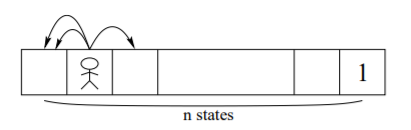
\includegraphics {pg_ex1}

Figure 3.1: policy gradient example 1 \\

The first example is the agent walking in the grid, and when it walk to the empty
grid, it can get the reward 0. And if it walk to the grid with number 1 (rightmost grid), it can get reward 1. And in this environment, two actions will move agent to the left and one action move agent to the right. For these class of problems, the expected time to reach the the goal state (reward 1 state) using undirected exploration \emph{ie} random walk exploration, is exponential in the size of the state space. And if the agent didn't reach the goal state in a trajectory, the estimate Q value will be 0, according to the policy gradient method, the estimate of the gradient will be 0, too. Which means that to obtain
a non-zero estimate of gradient, it requires exponential time with on-policy
samples.\\

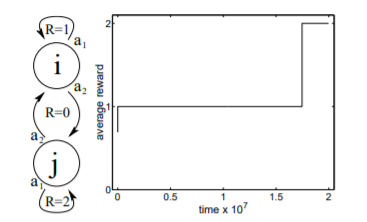
\includegraphics{pg_ex2}

Figure 3.2: policy gradient example 2 \\

And for the second example, there are two states state i and state j, And for each state there are two actions, a1 and a2. The initial distribution for this example will be:
\[ \rho(i) = 0.8, \; \rho(j) = 0.2 \]
And the policy of this example will be : \\
\[\pi(i,a1)=0.8, \; \pi(i,a2)=0.2, \; \pi(j,a1)=0.8, \; \pi(j,a2)=0.2\]
There is one assumption in this example, that the policy is using the common Gibbs table-lookup distributions:
\[{\pi_{\theta} \; : \;\pi(a;s) \; \propto \; exp(\theta_{sa})}\]
According to the discussion in [\cite{DBLP:ShipraAgrawalRLLecture7}], the $\theta_{s,a}$ can be updated by the following method:
\[\theta_{s,a} \gets \theta_{s,a} + \alpha d^{\pi}(s) \pi_{\theta}(s,a) 
(Q_{\pi}(s,a) - V_{\pi}(s))\]
Then we know that for state $i$, because $Q_{\pi}(i, a1)$ is bigger than 
$Q_{\pi}(i, a2)$ and $\pi(i,a1)=0.8$ is bigger than$ \pi(i,a2)=0.2$, too. So
the $\theta_{i,a1}$ will increase faster than $\theta_{i,a2}$, which make the
policy stay more times on state $i$. For state $j$, $\theta_{j,a1}$ increase more, but because of the initial distribution  $\rho(i) = 0.8 > \rho(j) = 0.2$, the policy will favor update at state $i$ but not state $j$. The analysis above
shows that learning at state $i$ reduces the learning at state $j$.
In Figure 3.2, we can observe an flat plateau at 1 average reward.

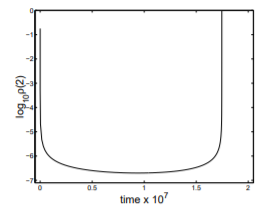
\includegraphics{pg_ex2-2}

Figure 3.3 \\

And Figure 3.3 shows the $\rho(j)$ become very low ($10^{-7}$) The author 
suggest that this example didn't give a good result to question 3. ("Which is 
concerned how fast such a policy can be found?") Because a gradient method could
end up trapped at the plateaus where estimating the gradient has an unreasonably
large sample complexity. \\

\newpage
\item Approximately optimal RL
\paragraph{Restart distribution \\}
According to two examples in the previous paragraph, the author shows that the policy gradient method may
not sensitive to some unlikely states, but these states may be important for finding the optimal policy.
So the author present another performance measure that can weight the improvement from all states more
uniformly:
\[\eta_{\mu}(\pi) \equiv E_{s{\thicksim}\mu} [V_{\pi}(s)]\]
Where $\mu$ is some "exploratory" \emph{restart distribution}. First the author wants to maximize $\eta_{\mu}$,
but maximize $\eta_{\mu}$ may have poor performance on $\eta_{D}$, so the author want to ensure that 
when maximize $\eta_{\mu}$ results in good policy under $\eta_{D}$. \\

\paragraph{Conservative policy update rule \\}
Then author present more conservative policy update rule:
\[\pi_{new}(a;s) = (1 - \alpha)\pi(a;s) + \alpha\pi'(a;s)\]
for some $\pi'$ and $\alpha \in 1$, $\pi'$ is the policy that is updated by greedy policy iteration based on 
some approximate state-action values. 
\\
Following subsections are about the main theorems of this paper. 

\paragraph{Policy improvement \\}
In this subsection, the author show that by finding some $\pi'$ that can make $\Delta \eta_{\mu}$ be positive, then the policy improvement occurs. And the author also present a theorem for the lower bound 
of the policy improvement.
\\
First, \textbf{policy advantage} is defined as:
\[A_{\pi,\mu}(\pi') \equiv E_{s{\thicksim}d_{\pi, \mu}} [E_{a{\thicksim}\pi'(a;s)} [A_{\pi}(s,a)]]\]
And by $\frac{\rho\eta_{\mu}}{\rho\alpha}|_{\alpha=0} = \frac{1}{1-\gamma}A_{\pi, \mu}$, the author shows that:
\[\Delta \eta_{\mu} = \frac{\alpha}{1 - \gamma}A_{\pi, \mu}(\pi') + O(\alpha^{2})\]
\\
So for the sufficiently small $\alpha$, policy improvement occur if policy advantage is positive.
By this observation, the author want to find the bound for the policy improvement, which is theorem 3.1:
\\
\paragraph{Theorem 3.1} (Theorem 4.1 in original paper)
\emph{Let $\mathbb{A}$ be the policy advantage of $\pi'$ with respect to $\pi$ and $\mu$. and let $\epsilon$ = $\max_{s}|E_{a{\thicksim}\pi'}(a;s)[A_{\pi}(s,a)]|$. For the conservative policy update rule and for all $\alpha \in [0, 1]:$}
\[\eta_{\mu}(\pi_{new}) - \eta_{\mu}(\pi) \geq \frac{\alpha}{1-\gamma} (\mathbb{A} - \frac{2\alpha\gamma\epsilon}{1 - \gamma(1 - \alpha)}) \]
\\

And the following corollary shows that the greater the policy advantage, the greater the guaranteed performance
increase.

\paragraph{Corollary 3.2} (Corollary 4.2 in original paper)
\emph{Let R be the maximal possible reward and $\mathbb{A}$ be the policy advantage of $\pi'$ with respect to $\pi$ and $\mu$. If $\mathbb{A} \geq 0$, then using $\alpha = \frac{(1 - \gamma)\mathbb{A}}{4R}$ guarantees the following policy improvement:}
\[\eta_{\mu}(\pi_{new}) - \eta_{\mu}(\pi) \geq \frac{A^{2}}{8R}\]
\\

The author didn't give a formal prove of this corollary, so I provide a prove in this report based on the author's hint : \\
First, based on the author's hint, I want to show that the change is bound by $\frac{\alpha}{1 - \gamma}
(\mathbb{A} - \alpha \frac{2R}{1 - \gamma})$:
By using the theorem 3.1, because $(1-\alpha) \leq 1$, we know that:

\begin{align*}
& \eta_{\mu}(\pi_{new}) - \eta_{\mu}(\pi) \\
& \geq \frac{\alpha}{1-\gamma} (\mathbb{A} - \frac{2\alpha\gamma\epsilon}{1 - \gamma(1 - \alpha)}) \\
& \geq \frac{\alpha}{1 - \gamma}(\mathbb{A} - \frac{2\alpha\gamma\epsilon}{1 - \gamma})
\end{align*}
\\

Because $\gamma \epsilon \leq \epsilon \leq \max_{s} |E_{a{\thicksim}\pi'}(a;s)[A_{\pi}(s,a)]| \leq R$, we know:

\[\frac{\alpha}{1 - \gamma}(\mathbb{A} - \frac{2\alpha\gamma\epsilon}{1 - \gamma}) \geq
\frac{\alpha}{1 - \gamma}(\mathbb{A} - \alpha \frac{2R}{1 - \gamma})\]

Then we prove that:
\[\eta_{\mu}(\pi_{new}) - \eta_{\mu}(\pi) \geq \frac{\alpha}{1 - \gamma}(\mathbb{A} - \alpha \frac{2R}{1 - \gamma})\]
\\

And the author also state that we need to choose $\alpha$ which maximize the bound, first I arrange the
right part to the quadratic form:
\[\frac{\alpha}{1 - \gamma}(\mathbb{A} - \alpha \frac{2R}{1 - \gamma}) = 
 - \frac{2R}{({1 - \gamma})^{2}} \alpha^{2} + \frac{\mathbb{A}}{1 - \gamma}\alpha \]
\\
 
Now we can see that the right part is a quadratic function, and we can find out the max value when it's
first derivative = 0:
\[- \frac{4R}{({1 - \gamma})^{2}} \alpha + \frac{\mathbb{A}}{1 - \gamma} = 0\]

Then solve for $\alpha$, when $\mathbb{A} \geq 0$:

\[ \alpha = \frac{(1 - \gamma)\mathbb{A}}{4R}\]
\\
\item Answer question 3 \\
The author address question 3 by first addressing how fast the policy converge and find the bound for
the quality of the policy.
First, the author access to an $\epsilon$ -greedy policy chooser to solve the problem. The algorithm
is called $\epsilon$-good algorithm $G_{\epsilon}(\pi, \mu)$ which is defined as:

\paragraph{Definition 3.3}
An \textbf{$\epsilon$-greedy policy chooser}, $G_{\epsilon}(\pi, \mu)$, is a function of a policy $\pi$
and a state distribution $\mu$ which returns a policy $\pi'$ such that $\mathbb{A}_{\pi,\mu}(\pi') \geq 
OPT(\mathbb{A}_{\pi,\mu}) - \epsilon$, where $OPT(\mathbb{A}_{\pi,\mu}) {\equiv} \max_{\pi'} \mathbb{A}_{\pi,\mu}(\pi')$. \\

Then the author introduce an outline of the main algorithm of this paper, \textbf{Conservative Policy Iteration}:\\
\begin{enumerate}[(1)]
\item Call $G_{\epsilon}(\pi, \mu)$ to obtain some $\pi'$. \\
\item Estimate the policy advantage $A_{\pi, \mu}(\pi')$ \\
\item If the policy advantage is small (less than $\epsilon$), STOP and return $\pi$. \\
\item Else, update the policy and go to (1). \\
\end{enumerate}

\newpage
Then the author start to solve question 3, "After a reasonable number of policy updates, what performance level is obtained?".\\ First, the author show that the algorithm satisfy the first condition
of the question, "A reasonable number of policy updates" by introduce Theorem 4.4:
\paragraph{Theorem 3.4} (Theorem 4.4 in original paper)
\emph{With probability at least 1 - $\delta$, conservative policy iteration: i)
improves $\eta_{\mu}$ with every policy update, ii) ceases in at most $72 
\frac{R^{2}}{\epsilon^{2}}$ calls to $G_{\epsilon}(\pi, \mu)$, and iii) return a policy $\pi$ such that $OPT(A_{\pi, \mu}) \leq 2 \epsilon$}. \\

And to bounds the performance of interest, which means answering "What performance level is obtained?" in question 3, the author gives Corollary 3.5.

\paragraph{Corollary 3.5} (Corollary 4.5 in original paper)
\emph{Assume that for some policy $\pi$, $OPT(A_{\pi}{\mu}) < \epsilon$. Let
$\pi*$ be an optimal policy. Then}
\[\eta_{D}(\pi*) - \eta_{D}(\pi) \leq \frac{\epsilon}{(1 - \gamma)} 
\left\Vert\frac{d_{\pi*, D}}{d_{\pi}{\mu}} \right\Vert_{\infty} \]
\[\leq \frac{\epsilon}{(1 - \gamma)^{2}}
\left\Vert \frac{d_{\pi*, D}}{\mu} \right\Vert_{\infty}\]
\\
By present theorem 3.4 and corollary 3.5, the author shows that the Conservative Policy Iteration can give a satisfactory answer to question 3. 
\\\\
And by corollary 3.2 and theorem 3.4, the author formally define the Conservative Policy Iteration as: \\

\begin{enumerate}[(1)]
\item Call $G_{\epsilon}(\pi, \mu)$ to obtain some $\pi'$ \\
\item Use $O(\frac{R^{2}}{\epsilon^{2}} log \frac {R^{2}}{\delta \epsilon^{2}})$
$\mu$-restarts to obtain an $\frac{\epsilon}{3}$ -accurate estimate $\hat{\mathbb{A}}$ of $\mathbb{A}_{\pi, \mu}(\pi')$. \\
\item If $\hat{\mathbb{A}} \frac{2\epsilon}{3}$, STOP and return $\pi$. \\
\item If $\hat{\mathbb{A}} \geq \frac{2\epsilon}{3}$, then update policy $\pi$ according to \textbf{Conservative policy update rule} using
$\frac{(1 - \gamma)(\hat{\mathbb{A}} - \frac{\epsilon}{3})}{4R}$ and return 
to step 1. \\
\end{enumerate}

\item Extension of the theorem 3.1\\
The theorem 3.1 proves the lower bound of the policy improvement, and I think it is also possible to give a upper bound to this improvement. \\
And to achieve this, I need a minor adjustment to the proof of theorem 3.1 from the original paper. Following is how I make this adjustment: \\
From the original proof, because $\Sigma_{a}\pi(a;s)A_{\pi}(s,a) = 0$ (proved in original paper), we know: \\
\[ E_{s {\thicksim} P}(s_{t};\pi_{new}) \bigg[\sum_{a} \pi_{new}(a;s) A_{\pi} (s,a) \bigg]\] \\
\[ = \alpha E_{s {\thicksim} P}(s_{t};\pi_{new}) \bigg[\sum_{a} \pi'(a;s) A_{\pi} (s,a) \bigg] \]
\[ = \alpha (1 - \rho_{t}) E_{s {\thicksim} P}(s_{t}|ct=0;\pi_{new}) \bigg[\sum_{a} \pi'(a;s) A_{\pi} (s,a) \bigg] \] 
\[+ \alpha \rho_{t} E_{s {\thicksim} P}(s_{t}|ct \geq 1;\pi_{new}) \bigg[\sum_{a} \pi'(a;s) A_{\pi} (s,a) \bigg]\]

And as the author stated in the paper, $Pr(ct = 0) = (1 - \alpha)^{t}$, and
$\rho_{t} \equiv Pr(c_{t} \geq 1) = 1 - (1 - \alpha)^{t}$, we know that:
\[ \alpha (1 - \rho_{t}) E_{s {\thicksim} P}(s_{t}|ct=0;\pi_{new}) \bigg[\sum_{a} \pi'(a;s) A_{\pi} (s,a) \bigg] \]
\[+ \alpha \rho_{t} E_{s {\thicksim} P}(s_{t}|ct \geq 1;\pi_{new}) \bigg[\sum_{a} \pi'(a;s) A_{\pi} (s,a) \bigg] \] 
\[\leq \alpha E_{s {\thicksim} P}(s_{t}|ct=0;\pi_{new}) \bigg[\sum_{a} \pi'(a;s) A_{\pi} (s,a) \bigg] + 2 \alpha \rho_{t} \epsilon \]
\[ = \alpha E_{s {\thicksim} P}(st;\pi)\bigg[\sum_{a} \pi'(a;s) A_{\pi} (s,a) \bigg] + 2 \alpha \rho_{t} \epsilon\] \\

Here the only change from the original proof is to change $- 2 \alpha \rho_{t} \epsilon$ to $+ 2 \alpha \rho_{t} \epsilon$ and the $\geq$ in third line to
$\leq$. Because we know that $\epsilon$ = $\max_{s}|E_{a{\thicksim}\pi'}(a;s)[A_{\pi}(s,a)]|$. So not only the lower bound
can be defined by adding $- 2 \alpha \rho_{t} \epsilon$ to the $\alpha E_{s {\thicksim} P}(st;\pi)\bigg[\sum_{a} \pi'(a;s) A_{\pi} (s,a) \bigg]$ , the upper bound can be found by adding $+ 2 \alpha \rho_{t}$
to $\alpha E_{s {\thicksim} P}(st;\pi)\bigg[\sum_{a} \pi'(a;s) A_{\pi} (s,a) \bigg]$.\\
And by changing $- 2 \alpha \rho_{t} \epsilon$ to $+ 2 \alpha \rho_{t} \epsilon$ in the original proof and lemma 6.1 in original paper, I get a policy improvement upper
bound, $\alpha \in [0, 1]$ and $\epsilon$ = $\max_{s}|E_{a{\thicksim}\pi'}(a;s)[A_{\pi}(s,a)]|$:
\[ \eta_{\mu}(\pi_{new}) - \eta_{\mu}(\pi) \leq \frac{\alpha}{1-\gamma} (\mathbb{A} + \frac{2\alpha\gamma\epsilon}{1 - \gamma(1 - \alpha)}) \]

Different from the original paper, this bound is represent the limitation for
a policy improvement.


\end{itemize}

 







